\chapter{State of The Art}



\section{Cryptography}
\subsection{Symmetric Encryption}
Symmetric Encryption and Asymmetric(public key) encryption are the two most common security mechanisms in place. Symmetric encryption entails the sending of an encrypted message to a receiver with use of a secret key. The same secret key is used in the decryption of the message. Before communication may begin with this design, a secure channel is necessary for both parties to declare a secret key to be used.

\subsection{Assymetric Encryption}
Asymmetric encryption entails the use of two different, but mathematically similar keys. Each party creates a public key, as well as a private key. The sender encrypts the message with their secret key, and the receiver may decrypt the message by using the public key of the sender. The involved parties in the process must have knowledge of eachother’s public keys. Whereas the distribution of private keys in symmetric encryption required a secure channel, in public key encryption only an authenticated channel is necessary as the public distribution of a user’s public key is not fatal to the design.

\section{Certificate Authorities}

\subsection{Background Of Certificate Authorities}
Certificate Authorities are third parties which are used for the purpose of validating the authenticity of public keys. A user’s public key is stored onto their digital certificate. The Certificate authority is responsible for the issuing, signing and verification of certificates. For a user to authenticate themself, a request is made to a certificate authority to issue a certificate to the user which is signed by the certificate authority’s private key. If another user receives a message containing this certificate, the user may see the signing of the CA and verify with them, the authenticity of the certificate and be sure that the certificate does belong to the sender.

\vspace{30pt}


\begin{center}
  \includegraphics[scale=.70]{CAOverview.png}
  \label{fig:Prob1:MEA}
\end{center}

\vspace{30pt}

Public key certificates are data structures which bind public key values to users. The binding is asserted by having a trusted CA digitally sign each certificate.

The structure for a 509 v3 certificate is a specified below:


\begin{center}
  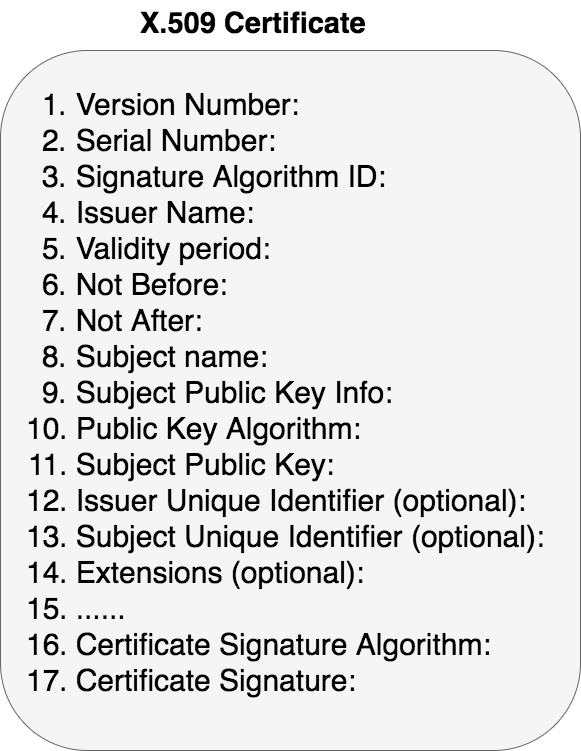
\includegraphics[scale=.5]{X509.png}
  \label{fig:Prob1:MEA}
\end{center}



\subsection{Issuing Of Certificates}

The method by which a CA verifies a users identity prior to signing a certificate lies in the means that the forms which CAs offer are either Domain Validated (DV) or Extended Validation (EV) SSL certificates.
\subsubsection{Domain Validated Certificates}

A Domain Validated certificate entails that a user creates a request for a certificate to be given by providing an email, a name and the domain for the certificate to be issued. The CA performs a whois lookup on the domain to check whether a user’s given name and email match what lies onto the domain’s registration information. Additionally, the CA may send an email to the email address to confirm that the user controls it. It is possible for this process to be completely automated and has been achieved after a string of companies created “Lets Encrypt”, an automated CA which offers DV certificates for free.

\subsubsection{Extended Validated Certificates}

An Extended Validated certificate requires a more detailed background search and requires human interaction. The certificate authority may require a phonecall, signed documents and a face-to-face meeting to verify a user's identity. The CA would confirm that the entity owns or has rights to use to a domain which they may wish to include in the certificate. Finally the CA confirms that the request for the EV has been authorised by the entity. The more thorough the validation process usually leads to a higher cost for the issuing of the certificate.

\subsection{Key Revocation}
Certificates are issued with the intention of being used for the enirity of their validation period. Loss of private key, change in users status or key comprimisation may lead to the certificate being revoced. Certificate authorities are responsible for the handling of certificates they issue after they have become comprimised. There are several methods such as Online Certificate Status Protocol (OCSP) and certificate revocation lists (CRLs) which are used to declare the revocation status of a certificate. Certificate revocation lists are the most common approach which is used.

A CRL is a list identifying all certificates which have been revoked by a CA. When a user interacts with a PKI system to identify another users identity, the user not only checks the certificate signature and validity but also checks the CRL to ensure that the certificate in question has not been revoked. An updated CRL is issued periodically by the CA. Once a certificate is revoked, it should appear on the next updated version of the CRL. To control growth, the certificate remains on the CRL until the certificate expires past it’s specificated validation period.

\subsection{Key Recovery}
In the event that a user loses their private key, after loss of device or accidental deletion, the user traditionally loses access to encrypt using their public key. In the design of PKI, the user has the option to allow the CA to backup the private key for them. This leads to an on-line protocol schemee where a user may later recover their lost key from the CA.


\subsection{Problems With Certificate Authorities}
A Certificate Authority is frequently described as “trusted”, however there is no reason for one to believe that a CA is entirely safe to use, other than the CA’s successful handling of private keys. This leads to the point that with an incredible number of CAs in the market today, it becomes increasingly difficult to identity the trustworthiness of each CA which a user encounters.

\subsubsection{Unassurace Of Certificate Quality}


As discussed, a more trustworthy CA requires more extensive background checks before issuing a certificate. This does not prevent users from acquiring certificates from more inexpensive authorities as certificates in the end may look identical other than the CA which had it issued. With the cost of creating a certificate in the perspective of a CA being low, many companies today issue certificates in large quantities at a low price. This lack of standard leads to a great unbalance of quality in the certificate ecosystem.

\subsubsection{Problems Of Authentication}

Certificates generally associate public keys with a person’s name. If one user receives a certificate from another user named “John Smith” and the CA confirms the validity of the certificate, this does not ensure that the “John Smith” named in the certificate is in fact the “John Smith” which the user knows. Further information about a user may be stored on the certificate to differentiate this “John Smith” from others on the CA , but it may be likey that the recipient is unsure of this information about the person, and furthermore not aware of which CA the certificate from their friend should come from.

\subsubsection{Certificate Validity Period}

As discussed, all certificates must contain a validity period which once expired, the certificate loses all of it’s uses. This is implemented to limit growth size of CRLs and to increase security by limiting the time that a certificate may be used by an attacker. Unfortunately this becomes abused by CA’s who take advantage of the need to reissue a certificate to clients and charge additional fees.

\subsubsection{Single Point Of Failure}
One of the most fundemental issues regarding the use of certificate authorities is that the decentralised nature of the design leads to a single point of failure at the certificate authority. This leads to total trust and dependance lieing on the stability and credibility of the CA. Attacks have occured, with the highest profile attack occuring in June 2011. DigiNotar, was a large Dutch certificate authority which was a primary certificate provider or domains owned by the dutch government. Afer a breach, an attack was able to issue more than 500 fradulent digital certificates on behalf of DigiNotar. The certificates issued were for some of the top internet companies such as Mozilla, Skype and Google. An attack of this nature led to the attacker to be able to pose their own sites and contain a certificate for another supposedly secure such as https://google.com. This would lead to users being at risk of sending their usernames and passwords to the attacker. DigiNotar lost all credibility following this attack and being unable to recover filed for bankruptcy two months later.
\section{Pretty Good Privacy And The Web Of Trust}
\subsection{Pretty Good Privacy}
Pretty Good Privacy(PGP) was first introduced in 1991 by Phil Zimmermann has become a standard for email security. The goal of PGP was to bring cyptography to the masses of people using the internet in an accesible manner.
\subsection{Confidentiality}
PGP combines both symmetric encryption and public key encryption to allow messages to be sent between users confidentially. The sender of a message creates a random symmetric key, and uses the symmetric key to encrypt the message to be sent. The sender then encrypts the key with the public key of the receiver. After both the encrypted message and key are sent to the receiver, the key can be decrypted with the receiver's private key, and the message decrypted by the symmetric key.

\begin{center}
  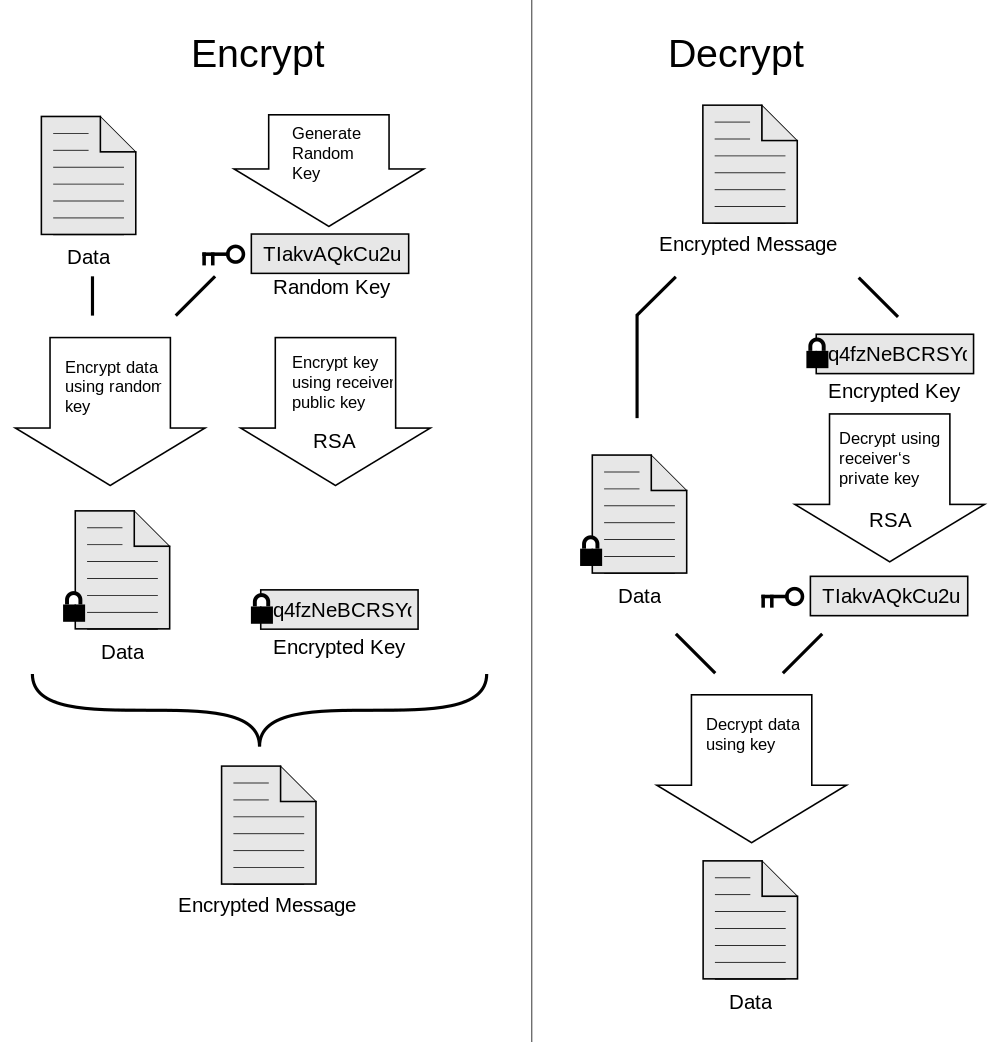
\includegraphics[scale=.25]{PGP.png}
  \label{fig:Prob1:MEA}
\end{center}

\subsection{The Web Of Trust}

In contrast to the hierarchical centralised approach of certificate authorites, PGP offers an alternative design by opting a "Web Of Trust" architecture. The central authority is removed, and it is the users who create the trust model. The user’s within the network possess the ability to sign other user’s keys, and view the signatures which a user has received. This builds a web of individual public keys, connected by links formed by these signatures.

Paul Zimmerman describes how the Web Of Trust may be used in the manual for PGP version 2.0 in 1992:

\textit{“As time goes on, you will accumulate keys from other people that you may want to designate as trusted introducers. Everyone else will each choose their own trusted introducers. And everyone will gradually accumulate and distribute with their key a collection of certifying signatures from other people, with the expectation that anyone receiving it will trust at least one or two of the signatures. This will cause the emergence of a decentralized fault-tolerant web of confidence for all public keys.”}

\begin{center}
  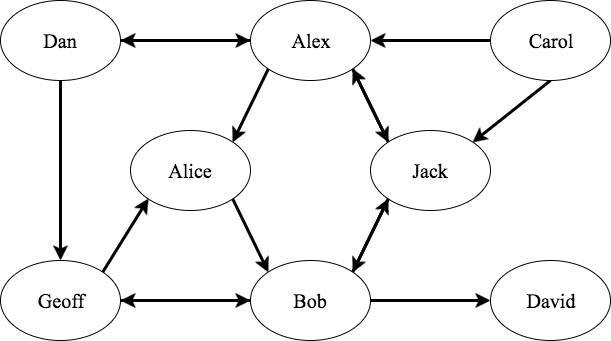
\includegraphics[scale=.75]{WOT_CONNECTION.png}
  \label{fig:Prob1:MEA}
\end{center}

\subsection{Key signing parties}
A key signing party is an event which is held whereby a large gathering of people occurs, where users meet to present their public key to others, and to have their key signed by them once the other person is confident that the key is authentic and belongs to that person. As the PGP infrastructure does not depend on a certificate authority to provide background check to authenticate others, signing parties act as a solution for users to become authenticated. The presenting of adequate identity documentation is required by participants at a key signing party prior to having their key signed.

\subsection{Establishing Trust}

The figure below shows Alice who is looking to communicate with Bob for the first time. Bob has had his colleague, Jack, sign his certificate which Jack knows is authentic. Alice knows Jack, and trusts Jack as an introducer. Alice can see that Jack has signed Bob’s certificate, therefore Alice can assume that Bob’s certificate is authentic. It is possible to have multiple signatures on a certificate, which may help in proving a certificate to be more trustworthy. However, had Alice had no introducer to Bob, it would be difficult for Alice to prove the authenticity of Bob.

\begin{center}
  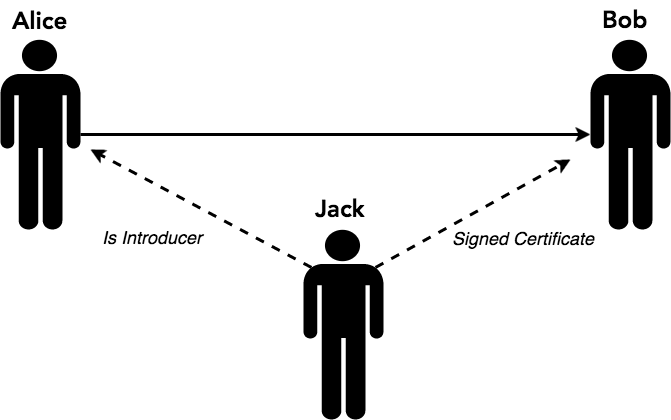
\includegraphics[scale=.6]{WOT.png}
  \label{fig:Prob1:MEA}
\end{center}

\subsection{Trustworthiness of Introducers}
To allow the system to become more reliable in determining the trustworthiness of  users, PGP allows for the rating of introducers to be split into three categories depending on the confidence attached to an introducer.
\begin{itemize}
  \item \textit{Full}: Full trust is one which you are fully confident in the introducer to only sign keys which are definitely trustworthy.
  \item \textit{Marginal}: Marginal trust entails that the introducer may be able to introduce you to a new user, but you may not be confident to always be trustworthy.
  \item \textit{Untrustworthy}: Untrustworthy introducers cannot be trusted in any case to introduce to new users.
\end{itemize}
Categorization of a user into one of these categories is not standard, and how to group an introducer into one of the categories is left entirely to the user themselves. PGP documentation does however offer guidelines for user to assist them in the vetting of  introducers.
\subsection{Trustworthiness of Users}

Public keys themselves can be split into three categories, where users can view the trustworthiness of the key without regard to their introducers.
\begin{itemize}
  \item \textit{Undefined}: It is not possible to tell whether the key is valid or not.
  \item \textit{Marginal}: The public key may be valid, but it is uncertain.
  \item \textit{Complete}: The public key is valid, and it is certain to be authentic.
\end{itemize}

With different levels of confidence placed on users, the Web Of Trust offers a mechanism for setting a number of both marginals trusts needed and complete trusts needed before a public key can become valid.

\subsection{Problems With The Web Of Trust}
PGP and the Web Of Trust prove to show a successful method to encrypted messages through email and various other applications. The decentralised architecture and removal of third party certificate authorities remove the single point of failures, reliance of trust on a CA and necessity for a valid lifetime on a public key. However, while it may not have the same shortcomings of the Certificate Authority architecture, PGP and the Web Of Trust unfortunately has flaws in it’s own.

\subsubsection{Key Loss}
While with Certificate Authorities, the loss of a user’s private key is not detrimental due to the ability for the Certificate Authority to securely backup a user’s key leading to no permanent loss of access to certificate. Due to the decentralised nature of PGP,  no key recoverability exists. If a user loses access to their private key, then the user must generate a brand new key pair. Due to the reputation aspect of the Web Of Trust, following key loss a user loses all signatures from their previous key,  and must generate a new reputation from scratch.

Loss of private key furthermore prevents a user from being able to decrypt messages, as well as move their public key to a key revocation list to prevent users from using it in future.

\subsubsection{Rating Of A User’s Trustworthiness}
The ambiguity of the nature of rating trust on users leads to an unbalance between the varying views which different users may perceive in rating the trustworthiness of a public key or an introducer.

\subsubsection{Entry Barrier For New Users}
One of the largest social obstacles in the design is in the large entry barrier which new users face. Upon creation of a new key pair, not having any signature on one’s key likely leads to not being readily trusted by other user’s systems which may require a certain number of introducers before authenticating a user.. The user must meet other users in person to authenticate themselves which may not always be possible. If a user is abroad and may never have an opportunity to meet those which they know, then it is unlikely that they will ever be able to become trusted.

\section{The Blockchain}
\subsection{The History Of The Blockchain}
\subsection{Introduction Of Bitcoin}

\section{Ethereum}
\subsection{History Of Ethereum}
\subsection{Smart Contracts}
